% This is the Reed College LaTeX thesis template. Most of the work 
% for the document class was done by Sam Noble (SN), as well as this
% template. Later comments etc. by Ben Salzberg (BTS). Additional
% restructuring and APA support by Jess Youngberg (JY).
% Your comments and suggestions are more than welcome; please email
% them to cus@reed.edu
%
% See http://web.reed.edu/cis/help/latex.html for help. There are a 
% great bunch of help pages there, with notes on
% getting started, bibtex, etc. Go there and read it if you're not
% already familiar with LaTeX.
%
% Any line that starts with a percent symbol is a comment. 
% They won't show up in the document, and are useful for notes 
% to yourself and explaining commands. 
% Commenting also removes a line from the document; 
% very handy for troubleshooting problems. -BTS

% As far as I know, this follows the requirements laid out in 
% the 2002-2003 Senior Handbook. Ask a librarian to check the 
% document before binding. -SN

%%
%% Preamble
%%
% \documentclass{<something>} must begin each LaTeX document
\documentclass[12pt,twoside]{reedthesis}
% Packages are extensions to the basic LaTeX functions. Whatever you
% want to typeset, there is probably a package out there for it.
% Chemistry (chemtex), screenplays, you name it.
% Check out CTAN to see: http://www.ctan.org/
%%
\usepackage{graphicx,latexsym} 
\usepackage{amssymb,amsthm,amsmath}
\usepackage{longtable,booktabs,setspace} 
\usepackage{chemarr} %% Useful for one reaction arrow, useless if you're not a chem major
\usepackage[hyphens]{url}
\usepackage{rotating}
\usepackage{natbib}
\usepackage{amsthm}
\usepackage[english]{babel}
\usepackage{float}
\usepackage{graphicx}
\usepackage{amssymb}
\usepackage{hyperref}
\usepackage[utf8]{inputenc}
\usepackage{listings}
\usepackage{pgf, tikz}
\usepackage{xcolor}
\usepackage{geometry}
\usepackage [english]{babel}
\usepackage [autostyle, english = american]{csquotes}
\MakeOuterQuote{"}
\geometry{margin=1in}
\usepackage[utf8]{inputenc}
\newtheorem{theorem}{Theorem}
\newtheorem{example}{Example}
\newtheorem{remark}{Remark}[section]
\newtheorem{definition}{Definition}[section]
\theoremstyle{definition}
\newcommand{\dsep}{\perp \!\!\!\perp}
% Comment out the natbib line above and uncomment the following two lines to use the new 
% biblatex-chicago style, for Chicago A. Also make some changes at the end where the 
% bibliography is included. 
%\usepackage{biblatex-chicago}
%\bibliography{thesis}

% \usepackage{times} % other fonts are available like times, bookman, charter, palatino

\title{My Final College Paper}
\author{Your R. Name}
% The month and year that you submit your FINAL draft TO THE LIBRARY (May or December)
\date{May 200x}
\division{Mathematics and Natural Sciences}
\advisor{Advisor F. Name}
%If you have two advisors for some reason, you can use the following
%\altadvisor{Your Other Advisor}
%%% Remember to use the correct department!
\department{Mathematics}
% if you're writing a thesis in an interdisciplinary major,
% uncomment the line below and change the text as appropriate.
% check the Senior Handbook if unsure.
%\thedivisionof{The Established Interdisciplinary Committee for}
% if you want the approval page to say "Approved for the Committee",
% uncomment the next line
%\approvedforthe{Committee}

\setlength{\parskip}{0pt}
%%
%% End Preamble
%%
%% The fun begins:
\begin{document}

  \maketitle
  \frontmatter % this stuff will be roman-numbered
  \pagestyle{empty} % this removes page numbers from the frontmatter

% Acknowledgements (Acceptable American spelling) are optional
% So are Acknowledgments (proper English spelling)
    \chapter*{Acknowledgements}
	I want to thank a few people.

% The preface is optional
% To remove it, comment it out or delete it.
    \chapter*{Preface}
	This is an example of a thesis setup to use the reed thesis document class.
	
	

    \chapter*{List of Abbreviations}

	

    \tableofcontents
% if you want a list of tables, optional
    \listoftables
% if you want a list of figures, also optional
    \listoffigures

% The abstract is not required if you're writing a creative thesis (but aren't they all?)
% If your abstract is longer than a page, there may be a formatting issue.
    \chapter*{Abstract}
	The preface pretty much says it all.
	
	\chapter*{Dedication}
	You can have a dedication here if you wish.

  \mainmatter % here the regular arabic numbering starts
  \pagestyle{fancyplain} % turns page numbering back on

%The \introduction command is provided as a convenience.
%if you want special chapter formatting, you'll probably want to avoid using it altogether

    \chapter*{Introduction}
         
	\chaptermark{Introduction}
	\markboth{Introduction}{Introduction}
	% The three lines above are to make sure that the headers are right, that the intro gets included in the table of contents, and that it doesn't get numbered 1 so that chapter one is 1.

% Double spacing: if you want to double space, or one and a half 
% space, uncomment one of the following lines. You can go back to 
% single spacing with the \singlespacing command.
% \onehalfspacing
% \doublespacing
	
	
    \chapter{The First}

\section{Background: Graphs, D-separation, Causality}
The idea of cause and effect has been studied and discussed in philosophy for centuries, but  the formalization of causality in mathematics, statistics, and computer science is much more recent. One framework in particular, Judea Pearl's Structural Causal Models (SCMs),  [ref Pearl 1996] is flexible, widely used, and mathematically elegant. However, before we can give SCMs a serious treatment, it is helpful to introduce definitions for the graphical machinery that most analysis of SCMs rely on.

\subsection{Directed Acylic Graphs}
\theoremstyle{definition}
\begin{definition}
A $\mathbf{graph}$ $G$ is a pair $G = (V, E)$ where $V$ denotes a set of nodes (sometimes called vertices) and $E \subseteq \{(i,j) | i,j \in V\}$ denotes a set of edges between nodes.
\end{definition}
Conventions differ, but for our purposes, an edge $(i,j) \in E$ is considered to be a \textbf{edge},  read as "an edge from node $i$ to node $j$".  For easy reading, we write $i \rightarrow j$ whenever $(i,j) \in E$. In the figures that frequently accompany graphs, an edge $(i,j)$ is depicted as an arrow from node $i$ to node $j$.

\begin{figure}
\centering
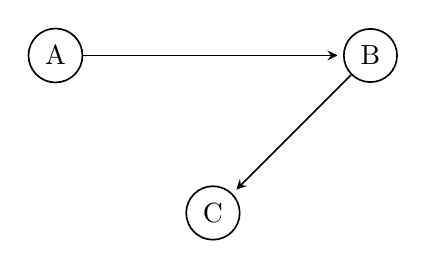
\begin{tikzpicture}[
            > = stealth, % arrow head style
            shorten > = 2pt, % don't touch arrow head to node
            auto,
            node distance = 3cm, % distance between nodes
            semithick % line style
        ]
\node[shape=circle,draw=black] (A) at (0,0) {A};
\node[shape=circle,draw=black] (B) at (4,0) {B};
\node[shape=circle,draw=black] (C) at (2,-2) {C};

 \path [->] (A) edge node[left] {} (B);
 \path [->] (B) edge node[left] {} (C);


\end{tikzpicture}
\caption{Graphs corresponding to $V = \{A,B,C\}$, $E = \{(A,B), (B,C)\}$ } \label{fig:M1}
\end{figure}

 Often times we are interested in how different nodes in a particular graph are or are not connected to one another. In this spirit we define paths.
 
\begin{definition}
A $\mathbf{path}$ $p$ between nodes $v_1, v_n \in V$ is a sequence $v_1, v_2, ..., v_n \in V$  of distinct nodes such that either $(v_i, v_{i+1}) \in E$ or $(v_i, v_{i+1}) \in E$ edge always exists between $v_i$ and $v_{i+1}$. When $v_i \rightarrow v_{i+1}$ ($(i, i-1) \in E$) for all $i \in \{1,2,...,n \}$, we say $p$ is a $\mathbf{directed \ path}$.
\end{definition}




For a directed graph $G$ and a particular node $v \in V$, we define several sets of related nodes. The \textbf{parents} of $v$, denoted $PA_v$, are the nodes with a directed edge ending at $v$, $\{j \in V | j \rightarrow v \}$ and similarly the \textbf{children}, denoted $CH_v$, of $v$ are those nodes which $v$ has a directed edge to, $\{j \in V | v \rightarrow j \}$. 

Extending these definitions, we define the \textbf{ancestors} of $v$, $AN_v$, as all the nodes from which a directed path to $v$ exists,  $\{j \in V | j \rightarrow ... \rightarrow v \}$. Likewise we define \textbf{descendants} $DE_v$ of $v$ as the nodes for which a directed path from $v$ exists,   $\{j \in V | v \rightarrow ... \rightarrow j\}$ [ref Peters chp 6.1]. With these in place, we progress to the next definition.

\begin{definition}
A directed graph $G = (V,E)$ is said to be an \emph{\textbf{directed acyclic graph}} (DAG) if for all nodes $v \in V$, $DE_v \cap AN_v = \emptyset$. That is, a directed graph is a DAG when there is never a directed path from a node to itself. 
\end{definition}

\begin{figure}
\centering
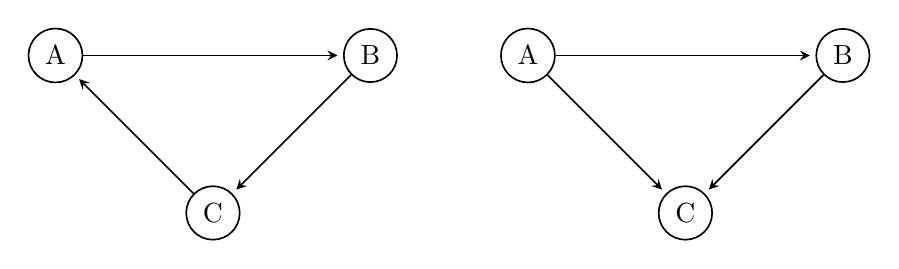
\begin{tikzpicture}[
            > = stealth, % arrow head style
            shorten > = 2pt, % don't touch arrow head to node
            auto,
            node distance = 3cm, % distance between nodes
            semithick % line style
        ]
\node[shape=circle,draw=black] (A) at (0,0) {A};
\node[shape=circle,draw=black] (B) at (4,0) {B};
\node[shape=circle,draw=black] (C) at (2,-2) {C};

 \path [->] (A) edge node[left] {} (B);
 \path [->] (B) edge node[left] {} (C);
  \path [->] (C) edge node[left] {} (A);


\node[shape=circle,draw=black] (A) at (6,0) {A};
\node[shape=circle,draw=black] (B) at (10,0) {B};
\node[shape=circle,draw=black] (C) at (8,-2) {C};

\path [->] (A) edge node[left] {} (B);
\path [->] (B) edge node[left] {} (C);
\path [->] (A) edge node[left] {} (C);
\end{tikzpicture}

\caption{Cyclic (left) and acyclic (right) graphs on the nodes $A,B,C$} \label{fig:M1}
\end{figure}

Now that we have defined DAGs, we can advance to a relevant application, Bayesian networks.

\subsection{Bayesian Networks}

Before we do so, we review some basic definitions from probability.

\begin{definition}
For random variables $X_1, X_2, ..., X_n$, the \textbf{joint distribution} with associated joint probability function $P(x_1, x_2, ..., x_n)$ gives the probability of every possible combination of values for $X_1, X_2, ..., X_n$. For any subset $\{Y_1,...,Y_k\} \subseteq \{X_1, X_2, ..., X_n\}$, the probability distribution for $Y_1, Y_2, ..., Y_k$, is called the \textbf{marginal distribution}. Finally, for a subset 
\end{definition}



\subsection{D-Separation}
Graphical structure can allow us to reason about causal and statistical relationships. One of the essential tools is d-separation. To develop the intuition, consider the very basic DAG $A \rightarrow B \rightarrow C$. There is exactly one directed path from $A$ to $C$, and the path passes through $B$. So to get to $C$ from $A$ you need to pass through $B$. In this way, we say that $B$ blocks the directed path from $A$ to $C$. We extend this notion [ref Pearl 2008], [ref Peters 2017].

\begin{definition}
Given a directed graph $G$, a path $p$ from node $v_1$ to node $v_n$ is said to be \textbf{\emph{blocked}} by a set $S$ (with $S \cap \{v_1, v_n\} = \emptyset$) if:
\begin{enumerate}
\item $v_j \in S$ and $p$ contains a $\mathbf{chain}$: $v_{j-1} \rightarrow v_j \rightarrow v_{j+1}$ or $v_{j-1} \leftarrow v_j \leftarrow v_{j+1}$, or

\item $v_j \in S$ and $p$ contains a \textbf{\emph{fork}}: $v_{j-1} \leftarrow v_j \rightarrow v_{j+1}$, or

\item $v_j \notin S$ and $DE_{v_j} \cap S = \emptyset$ and $p$ contains a \textbf{\emph{collider}}: $v_{j-1} \rightarrow v_j \leftarrow v_{j+1}$. As we will see, colliders play an especially important role in the analysis of causal DAGs.
\end{enumerate}
\end{definition}

\begin{example}
Consider a path $A \rightarrow B \rightarrow C \leftarrow D \rightarrow E$ between nodes $A$ and $E$. There are many sets that block this path. For one, there is a collider on the path. This means that any set which does not include $C$ or any elements of $DE_C$ would successfully block the path. However, we could also pick $S = \{B\}$, $S= \{D\}$, or $S = \{B,D\}$ as blocking sets since the path contains a chain at $B$ and a  fork at $D$. Importantly, if we have either of these nodes in our blocking set, we could include $C$ as well because the first blocking condition would be satisfied, even though the second would not. In fact, the only $S \subseteq \{B,C,D\}$ that would not block the path is $S = \{C\}$.
\end{example}

With blocking defined, we address d-separation. 

\begin{definition}
For a DAG $G$, two sets of nodes $A,B \in G$ are said to be  \textbf{\emph{d-separated}} by a set $S$ if all paths between $A$ and $B$ are blocked by $S$. We denote d-separation by the symbol $\perp \!\!\!\perp_G$, with the statement "In DAG $G$, $A$ is d-separated from $B$ by $S$" expressed as $A \dsep_G B | S$. 
\end{definition}

\begin{remark}
If $A \dsep_G B | S$ then $B \dsep_G A | S$
\end{remark}
\begin{example}
Consider the DAG $G$ below.

    $$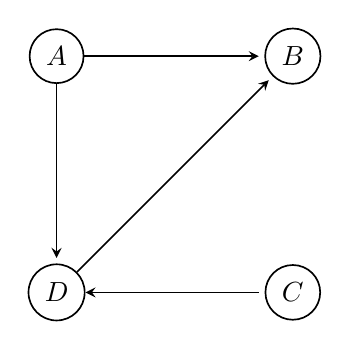
\begin{tikzpicture}[
            > = stealth, % arrow head style
            shorten > = 2pt, % don't touch arrow head to node
            auto,
            node distance = 3cm, % distance between nodes
            semithick % line style
        ]
        

        \tikzstyle{every state}=[
            draw = black,
            thick,
            fill = white,
            minimum size = 4mm
        ]

        \node[shape=circle,draw=black] (A) {$A$};
        \node[shape=circle,draw=black] (B) [right of=A] {$B$};
        \node[shape=circle,draw=black] (C) [below of=B] {$C$};
        \node[shape=circle,draw=black] (D) [left of=C] {$D$};

        \path[->] (A) edge node {} (B);
	    \path[->] (A) edge node {} (D);
	    \path[->] (D) edge node {} (B);
	    \path[<-] (D) edge node {} (C);
    \end{tikzpicture}$$
\end{example}

Which nodes can be d-separated, and by which blocking sets? Nodes which are connected by an edge cannot be d-separated. To see why, take $A$ and $B$. Although some paths between $A$ and $B$ can be blocked, the path $A \rightarrow B$ contains no nodes other than $A$ and $B$ and therefore cannot be blocked. Since there is no set that can block the path, $A$ and $B$ are not able to be d-separated. So consider $A$ and $C$, two nodes which are not connected by an edge. There are two paths between $A$ and $C$, $A \rightarrow B \leftarrow D \leftarrow C$ and $A \rightarrow D \leftarrow C$. Both of these paths include a collider. Of the four possible blocking sets, $\emptyset, \{B\}, \{D\}, \{B,D\}$, all but $\emptyset$ include a collider node for paths that are not blocked by other means. Then $A \dsep_G C | \emptyset$ and no other sets will work. What about $B$ and $C$? Again there are two paths: $B \leftarrow D \leftarrow C$ and $B \leftarrow A \rightarrow D \leftarrow C$. The second path contains a collider, and therefore is blocked by $\emptyset$, but the first path cannot be. To block $B \leftarrow D \leftarrow C$ we must have $D$ in our blocking set. So, $B \dsep_G C | D$, but we can also include $A$ since doing so will not unblock a path with a collider. Then $B \dsep_G C | D,A$.


\subsection{Structural Causal Models}
Many questions in the natural and social sciences involve understanding the way that one set of factors (e.g. genes, medicines, social policies) influence others (e.g. disease risk, mortality, childhood poverty rates). In these cases, the language and  of classical statistics is often inadequate. The tools of hypothesis testing, (linear) regression, interval estimation, etc. can tell us much about relationships in the data, but except in the highly constrained setting of randomized controlled trials, very little about cause and effect. These limitations are not just theoretical. Many longstanding controversies and debates within the sciences come down to disagreements over which factors associated with a particular outcome are causing the outcome. 

A paradigmatic example of such a controversy is over the relationship between cigarette smoking and lung cancer. Today, it is uncontroversial that smoking cigarettes (especially habitually over a long period of time) increases a person's risk of contracting lung cancer. This is a causal relationship, and we might express our belief in this relationship as a \textbf{\emph{causal model}} in which a person's risk of contracting lung cancer is a \emph{function} of a person's smoking habits (for simplicity, we  pretend that smoking is the only such causal factor).

So, let $L$ be a random variable denoting whether or not a person contracts lung cancer and $S$ be a random variable denoting smoking. Under our causal model in which smoking is the only structural cause of lung cancer, we express $L$ as a function of $S$:

$$L :=f(S, N_L),$$
$$S := N_S.$$ 

Here, the use of $:=$ denotes an assignment rather that an algebraic relationship [ref Peters] and $N_L$ is a noise term capturing random effects on lung cancer risk, and $N_S$ a noise variable for cigarette smoking. Together, these two assignments are a  structural causal model.  Now that we have an SCM, we can express the structure as a DAG. Since $L$ is assigned as a function of smoking but $S$ is not caused by any factors in our model, we would express our model as a directed edge going from $S$ to L:



$$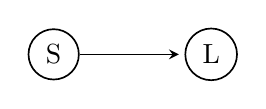
\begin{tikzpicture}[
            > = stealth, % arrow head style
            shorten > = 2pt, % don't touch arrow head to node
            auto,
            node distance = 3cm, % distance between nodes
            semithick % line style
        ]
\node[shape=circle,draw=black] (S) at (8,0) {S};
\node[shape=circle,draw=black] (L) at (10,0) {L};


 \path [->] (S) edge node[left] {} (L);
\end{tikzpicture}$$

However, historically, this causal structure was not the only one suggested to explain the association between lung cancer and smoking. One particularly illustrious detractor of this theory was British statistician R. A. Fisher, a foundational figure in modern statistics (and a heavy smoker) [ref Fisher]. In Fisher's view, there was no causal effect of smoking on lung cancer, rather, an underlying genetic factor was responsible for both a predisposition to smoking and a higher risk of developing lung cancer. So Fisher's causal model would have looked like:
$$L :=f(G, N_L),$$
$$S := f(G, N_S),$$
$$G := N_G.$$ 
Where $G$ is the genetic factor. As before, the structure of this model can be expressed as a graph:

$$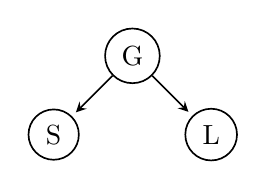
\begin{tikzpicture}[
            > = stealth, % arrow head style
            shorten > = 2pt, % don't touch arrow head to node
            auto,
            node distance = 3cm, % distance between nodes
            semithick % line style
        ]
\node[shape=circle,draw=black] (G) at (9,1) {G};
\node[shape=circle,draw=black] (S) at (8,0) {S};
\node[shape=circle,draw=black] (L) at (10,0) {L};

 \path [->] (G) edge node[left] {} (L);
 \path [->] (G) edge node[left] {} (S);
\end{tikzpicture}$$


In this way, every SCM entails a directed graph. Although it is entirely possible for an SCM to entail a graph that has cycles, we focus our attention on the case where the graph entailed is a DAG. Importantly, these two (graphical) models imply different observational joint distributions. Without having specified the functions, little can be said about the joint distribution entailed by the model, however, one important property is built in to every SCM.

\begin{definition}[Markov property]
In any SCM $C$ with entailed graph $G$, if $A \dsep_G B | S \implies A \dsep B | S$ for all disjoint sets of nodes $A,B,S$. That is, every d-separation in the graph corresponds to a conditional independence in the joint distribution. This fact is implied by the definition of SCMs and is called the \emph{\textbf{Markov Property}}.
\end{definition}

[This seems important enough to reproduce a proof but I will have to spend a little more time than I have tonight]

This result is a powerful tool that allows us to test how well differing causal models comport with the observational data.  Returning to Fisher's suggestion that an underlying genetic cause was responsible for the association of smoking with lung cancer, consider that by the Markov property $S \dsep L | G$. Let's assume we have a population of identical twins, some of whom were smoking discordant. Since we know that identical twins are genetically identical  we could assess whether or not smoking and lung cancer are independent within twin pairs. If not, then something must be wrong with the model. 
	

 \chapter{Bareinboim et al 2014}


\section{Introduction}
Bareinboim, Tian, and Pearl's 2014 paper "Recovering from Selection Bias in Causal and Statistical Inference" provides a formulation of selection bias explicitly in terms of causal DAGs and d-separation, making it an especially important resource for developing our study of the topic. In particular, the paper provides graphical conditions (in terms of d-separations) under which a \emph{conditional} distribution $P(y | x)$ can be obtained despite selection bias. When this can be done, we say that the $P(y | x)$ can be "recovered", from a causal graph containing a selection mechanism. However, the content of the paper is highly abstracted and does not attempt to provide real-life cases in which their techniques are useful. For this reason, we will summarize the main results of the paper and interpret them in the context of some realistic examples. 

The paper is broken into three sections, the first two of which are the most substantial and the focus of our attention. The first gives conditions for when a distribution can be recovered if only the biased distribution is accessible, the second gives conditions for the case where population level data is available for some variables, and the last gives a brief discussion of recovering causal effects.

\section{Representing Selection with DAGs}

Although the topic of this paper is selection \emph{bias}, the graphical framework is really a model of selection itself. That is, it can model cases where selection does not induce bias as well as cases in which it does. Representing selection in this way requires augmenting  a structural causal model over a set of variables $\mathbf{V}$ with a node $S$ that represents inclusion in the sample. The biased distribution is then $P(\mathbf{v} | S = 1)$, that is, the joint for our variables $\mathbf{V}$ conditioned on inclusion within the sample.  

\section{A Famous Case of Selection Bias}
One classic example of selection bias is the 1936 presidential election poll  published in an American magazine called The Literary Digest. The election was between Franklin Delano Roosevelt, the democratic incumbent, and Alfred Landon, a republican. The Literary Digest conducted a poll, drawing from their readership and by telephone and using records of automobile ownership. The sample size was extremely large, with over 2 million survey respondents. Their prediction, that Landon would comfortably win the election, proved embarrassing. Not only did Landon lose, but he lost in one of the largest electoral landslides in American history:  523 electoral votes went to Roosevelt and 8 went to the Digest's predicted winner. Shortly after, the magazine ceased publication.

The precise details of what caused this failure are not fully known. One view that has become the popular explanation was that although their survey had a plenty large sample size, it was non-representative of the population as a whole. Particularly, both being subscribed to The Literary Digest and owning a telephone or car were more common among more affluent people, and so their survey skewed wealthier than the population as a whole, and therefore underestimated the proportion of voters who would vote for Roosevelt, a candidate with largely working class support. In fact, this explanation is unlikely to be complete. Although it is true that the survey over-sampled more affluent voters who were more likely to support Landon, a separate poll  conducted by George Gallup in 1937 found that in even voters who owned both a telephone and a car were more likely to favor Roosevelt than Landon. This means that there must have been other factors at play, and in particular, that Landon voters were more likely to return the survey than Roosevelt voters \citep{Squire1988}, \cite{lusinchi_2012}. This is called (non) response bias, and we will see that it falls under the selection bias framework proposed here.

For now, though, let's assume that income was the only variable that was responsible for the non-representative sample, and that this information was collected from respondents as part of the survey. However, we will return to this case later to add some depth.

One of the important features of selection bias is that unlike sampling variation, it cannot be reduced with sufficiently large sample sizes. For this reason, in the rest of the paper we will discuss a selection biased joint distribution for this survey, and thereby ignore sample size.

\section{Recovering $P(y|x)$ Without External Data}
In the simplest case, we only have access to a distribution corresponding to a causal graph $G$  with a set of nodes $\mathbf{V}$ equipped with a selection node $S$. This means that we do not have access to the full joint distribution $P(\mathbf{v})$ but rather the conditional joint distribution $P(\mathbf{v} | S = 1)$. This corresponds to the joint distribution of values that are selected to be sampled. So, returning to our election example, our graph would look like:
\begin{figure}
\begin{center}
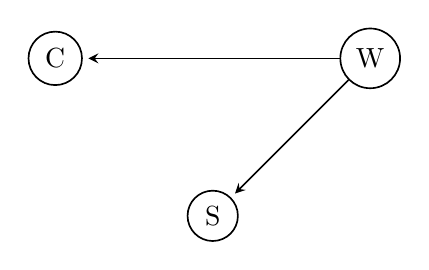
\begin{tikzpicture}[
            > = stealth, % arrow head style
            shorten > = 2pt, % don't touch arrow head to node
            auto,
            node distance = 3cm, % distance between nodes
            semithick % line style
        ]
\node[shape=circle,draw=black] (C) at (0,0) {C};
\node[shape=circle,draw=black] (W) at (4,0) {W};
\node[shape=circle,draw=black] (S) at (2,-2) {S};

 \path [->] (W) edge node[left] {} (S);
 \path [->] (W) edge node[left] {} (C);

\end{tikzpicture}
\end{center}
\caption{Graph corresponding to selection bias based on income} \label{fig:2.1}
\end{figure}
Where $C$ is a random variable for the candidate a person intends to vote for, $W$ is measures income and $S$ is a binary variable denoting inclusion in the study. Although in practice we would probably like to know $P(c)$, the population level distribution of intended votes, for now we restrict ourselves to $P(c | w)$, the conditional distribution of intended vote given SES. 

In the vein, Bareinboim et al. define \textbf{s-recoverability} as the criterion which must be satisfied for a conditional distribution such as $P(c|w)$ to be obtainable under selection bias. We reproduce their definition exactly and give an explanation of why it makes sense.

\begin{definition}
Given a causal graph $G_s$ augmented with a node $S$ encoding the selection mechanism, the distribution $Q = P(y | \mathbf{x})$ is said to be \textbf{s-recoverable} from selection biased data in $G_s$ if the assumptions embedded in the causal model render $Q$ expressible in terms of the distribution under selection bias $P(\mathbf{v} | S = 1)$. Formally, for every two probability distributions $P_1$ and $P_2$ compatible with $G_s$, $P_1(\mathbf{v} | S = 1) = P_2(\mathbf{v} | S = 1) > 0$ implies $P_1(y | \mathbf{x}) = P_2(y | \mathbf{x})$.
\end{definition}

If we have a selection biased distribution, we have access to a particular joint distribution, $P(\mathbf{v} | S = 1)$ where $\mathbf{V}$ is the set of all nodes other than $S$. So if we are to recover $P(y | \mathbf{x})$ ($\mathbf{X} \subset \mathbf{V}$, $Y \in \mathbf{V}$) we need to express $P(y | \mathbf{x})$ as values derivable from $P(\mathbf{v} | S = 1)$ and the conditional independences implied by the d-separations within the graph. This is what is meant by "if the assumptions embedded in the causal model render $Q$ expressible in terms of the distribution under selection bias $P(\mathbf{v} | S = 1)$", and it is worth exploring why this fairly intuitive formulation is equivalent to the formal definition given in the last sentence.

Consider that the agreement of $P_1$ and $P_2$ on the joint distribution $P(\mathbf{v} | S = 1)$ means that $P_1$ and $P_2$ produce the same observational distribution under selection bias. Therefore, when $P_1(\mathbf{v} | S = 1) = P_2(\mathbf{v} | S = 1) \implies P_1(y | \mathbf{x}) = P_2(y | \mathbf{x})$ we know that no matter the differences between $P_1$ and $P_2$, they must produce the same conditional $P(y|\mathbf{x})$. So, if this is true for every $P_1$, $P_2$, then all distributions consistent with the observational $P(\mathbf{v} | S = 1)$ produce the same $P(y | \mathbf{x})$. 
The first important result of the paper is the following theorem:
\begin{theorem}
The distribution $P(y | \mathbf{x})$ is s-recoverable from $G_s$ if and only if $S \dsep_{G_s} Y | \mathbf{X}$.
\end{theorem}

The proof of $\impliedby$ is quite long, but $\implies$ is easy. 

\begin{proof}
Assume that $S \dsep_{G_s} Y | \mathbf{X}$. Then by the Markov property, $S \dsep Y | X$ and $P(y | \mathbf{x}, S = 1) = P(y | \mathbf{x})$. So the 'recovered' distribution is simply the biased distribution.
\end{proof} 

Clearly this is a useful result since it is easy to test whether two nodes are d-separated by a set. In our application, we can see that $V \dsep_G S | W$, and so $P(v|w) = P(v|w, S = 1)$. So our study gives us direct access to the conditional distribution for candidate preference by income. This is potentially useful but restricted. What if we wish to recover a conditional distribution but do not want to condition on the full separating set? To do so, we will need external measurements.

\section{Recovery With External Data}

Sometimes a researcher will conduct a survey and collect variables on survey participants for which we know the population level distribution. For instance, the US Census collects and publishes data on occupation, race, income, and many other variables from the entire US population. If some of these variables are measured in our selection biased study, this information can be used to recover distributions that would otherwise be unavailable. To elaborate on this topic we will introduce a more complex model of the selection mechanism in our voter poll. As mentioned in the introduction, more recent research suggests that the assumption that income was the only variable affecting the probability of being included in the poll is not sufficient. A better explanation includes the fact that Roosevelt supporters who received the survey were much less likely to respond than Landon supporters \cite{lusinchi_2012}. This effect is called non-response bias, and is really another form of selection bias since it arises from the differing probabilities of being included in the final sample. The exact mechanism of the non-response effect in this poll is not and likely will never be known. In fact, if candidate preference directly influences the likelihood of survey response, (i.e. $C \rightarrow S$), the two nodes cannot be d-separated and we will be out of luck. Being optimistic, however, let's say we have reason to believe that another factor is the culprit. Particularly, the political party to which a survey respondent is registered could be mediating the relationship between voter preference and response probability. This model is represented in the figure below.


\begin{figure}
\begin{center}
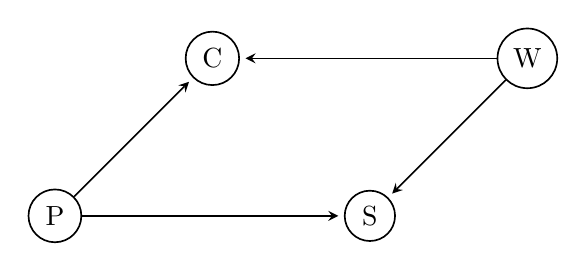
\begin{tikzpicture}[
            > = stealth, % arrow head style
            shorten > = 2pt, % don't touch arrow head to node
            auto,
            node distance = 3cm, % distance between nodes
            semithick % line style
        ]
\node[shape=circle,draw=black] (C) at (0,0) {C};
\node[shape=circle,draw=black] (W) at (4,0) {W};
\node[shape=circle,draw=black] (P) at (-2,-2) {P};
\node[shape=circle,draw=black] (S) at (2,-2) {S};


 \path [->] (P) edge node[left] {} (S);
  \path [->] (W) edge node[left] {} (S);
 \path [->] (P) edge node[left] {} (C);
 \path [->] (W) edge node[left] {} (C);
\end{tikzpicture}
\end{center}
\caption{Graph corresponding to selection bias based on income and party registration} \label{fig:2.1}
\end{figure}

Where $P$ is a binary variable denoting the party registration status of the voter. Under this model, we have a path $S \leftarrow U \rightarrow V$ which is not blocked by $W$. So $S \not \dsep_G Y | X$ and by the previous theorem, we cannot recover $P(c|w)$. Of course, we could recover $P(c | w, p)$ since $S \dsep_G V | \{W,P\}$, but assuming we are still interested in $P(c|w)$, what can be done?  

Well, we could consult the US census as well as state voter records and gather the  joint distribution for income and party registration $P(u, w)$. This is what we would call \emph{external data} since it is not affected by the selection mechanism. It turns out that in this case, we can do something. To address this situation, Bareinboim et al.  introduce a revised definition  of s-recoverability which we again reproduce and comment on. 
 
\begin{definition}
Given a causal graph $G_s$ augmented with a node $S$ encoding the selection mechanism, the distribution $Q = P(y | \mathbf{x})$ is said to be \textbf{s-recoverable} from selection bias in $G_s$ with external data over $\mathbf{T} \subseteq \mathbf{V}$ and selection biased data over $\mathbf{M} \subseteq \mathbf{V}$ if the the assumptions embedded in the causal model render $Q$ expressible in terms of the distribution under selection bias $P(\mathbf{m} | S = 1)$ and $P(\mathbf{t})$, both positive. Formally, for every two probability distributions $P_1$ and $P_2$ compatible with $G_s$, if they agree on the available distributions $P_1(\mathbf{v} | S = 1) = P_2(\mathbf{v} | S = 1) > 0$, $P_1(\mathbf{t}) = P_2(\mathbf{t})$ they must agree on the query distribution $P_1(y | \mathbf{x}) = P_2(y | \mathbf{x})$.
\end{definition}

We can see that this definition follows the same structure as the original s-recoverability definition, but is expanded to allow for the use of population level distributions. The paper's second theorem follows directly from this definition.

\begin{theorem}
If there is a set $C \subseteq V$ such that $P(\mathbf{c}, \mathbf{x})$ is measured in the population and $Y \dsep_{G_s} S | \{C,X\}$ then $P(y | \mathbf{x})$ is s-recoverable as

$$P(y | \mathbf{x}) = \sum_{\mathbf{c}} P(y | \mathbf{x}, \mathbf{c}, S = 1)P(\mathbf{c} | \mathbf{x})$$
\end{theorem}

The theorem is a straightforward application of the law of total probability.
\begin{proof}
By assumption, we have the external distribution $P(\mathbf{c}, \mathbf{x})$ and therefore $P(\mathbf{c} | \mathbf{x})$, and as usual we have $P(\mathbf{v} | S =  1)$. So can apply the law of total probability and the conditional independence $Y \dsep S | \{C,X\}$ to write:

$$P(y | \mathbf{x}) = \sum_{\mathbf{c}} P(y | \mathbf{x}, \mathbf{c}) P(\mathbf{c} | \mathbf{x}) = \sum_{\mathbf{c}} P(y | \mathbf{x}, \mathbf{c}, S = 1) P(\mathbf{c} | \mathbf{x})$$

\end{proof}

Therefore, if we wish to recover $P(c | w)$ party registration affects response probability, we can do so using the external data $P(p | w)$.

\section{A Useful Extension}
As we have seen, Bareinboim et al. is focused on the recovery of conditional distributions, i.e. $P(v|w)$. However, we would often like to have the unconditional distribution $P(v)$. Although it is only mentioned obliquely at the end of the second section, the results they prove give a simple condition for when $P(v)$ is recoverable using external data. In both sections we have seen that $P(v|w)$ was recoverable. Then, assuming that we have the external data for $P(w)$, we can use the law of total probability to write:

$$P(v) = \sum_{w} P(v|w)P(w).$$

More generally, we can formulate this result as a theorem, although it is not listed as such in the paper.

\begin{theorem}
If there exists a set $\mathbf{X} \subseteq V$ such that $P(y|\mathbf{x})$ is s-recoverable and $P(\mathbf{x})$ is available externally, then $P(y)$ is recoverable as $P(y) = \sum_{\mathbf{x}} P(y|\mathbf{x})P(\mathbf{x})$.
\end{theorem}

\chapter{Graphical Approaches to Missing Data}

We have seen that selection bias is one way that the data collection process can cause the available distribution to differ from the desired distribution. A closely related problem (which is occasionally referred to as selection bias) is the problem of missing data \citep{Heckman_1979}. This happens often in statistical practice: survey question non-response, study drop-out, and failing to record data are all well known forms of missingness that affect scientific research. 

Missing data occurs when some variables are not observed for each unit (row). In the standard missing data notation, $R_{Y_i}=1$ corresponds to the $i^{\text{th}}$ observation of a random variable $Y$ being missing. Missingness can follow a very simple structure where a particular variable is not always observed (often the response variable), but covariates are available for each unit. Table 3.1 gives an example of what is meant by this. 


\begin{table}[]
\centering
\begin{tabular}{|l|l|l|l|l|l|}
Y     & $X_1$  & $X_2$  & $X_3$  & $X_4$  & $R_Y$ \\ \hline
$y_1$ & $x_{11}$ & $x_{12}$ & $x_{13}$ & $x_{14}$ & 0 \\
   -   & $x_{21}$ & $x_{22}$ & $x_{23}$ & $x_{24}$ & 1 \\
   -   & $x_{31}$ & $x_{32}$ & $x_{33}$ & $x_{34}$ & 1 \\
$y_2$ & $x_{41}$ & $x_{42}$ & $x_{43}$ & $x_{44}$ & 0
\end{tabular}
\caption{Hypothetical table representing missing data with one partially observed variable.} 
\end{table}

One example of this effect is found in studies that observe units over a long period of time. In these cases, researchers often have to deal with drop-out: some participants stop participating in the study before it finishes, and therefore the final outcome is not recorded for these units. Since the pre-treatment covariates are recorded for all participants before dropout occurs, only the outcome variable is missing for the units affected by dropout. This situation is a prime candidate for a technique called inverse probability weighting, which we explore in the next chapter \citep{Hernan_2004}.

Sometimes the missingness structure is more complex in that different variables are missing from different units. A range of approaches have been developed: sometimes, rows with missing variables may be safely deleted, other times, imputation base methods are more appropriate \citep{Schafer_2002}.  For instance, survey respondents may choose not to answer some questions, but unlike in the example above, the unanswered questions can differ between units (table 3.2). In cases like this, missing data are often imputed: that is, the missing values are predicted on the basis of non-missing values, but weight based approaches like inverse probability weighting can also be applied \citep{Little_1986} ,\citep{Seaman_2011}. 

\begin{table}[]
\centering
\begin{tabular}{|l|l|l|l|l|l}
$X_1$    & $X_2$    & $X_3$    & $R_{X_1}$ & $R_{X_2}$ & $R_{X_3}$ \\ \hline
-        & -        & $x_{13}$ & 1         & 1         & 0         \\
-        & $x_{22}$ & $x_{23}$ & 1         & 0         & 0         \\
$x_{31}$ & $x_{32}$ & $x_{33}$ & 0         & 0         & 0         \\
-        & $x_{42}$ & -        & 1         & 0         & 1        
\end{tabular}
\caption{Hypothetical table representing missing data with all variables partially observed.}
\end{table}

Since such a wide range of missingness structures are possible, a large  literature has developed to address the problem in various contexts \citep{Schafer_2002}.  However, a taxonomy developed  by Donald Rubin to capture the basic structures under which missingness occurs has had a particularly notable impact. We review these definitions now, since our graphical framework will also make use of them. 

\section{Rubin's Taxonomy of Missing Data}

Donald Rubin's work on the missing data problem is likely the most influential out of any researcher on the topic. Rubin developed several notable techniques to address missing data including multiple imputation, the expectation-maximization algorithm, and the theory of propensity scores \citep{Little_1986}. We will discuss these methods in more details later in the next chapter, but Rubin's taxonomy \citep{Rubin_1976} of the structure of missingness is important enough to introduce now. Consider a  case with a set of variables $V_m$ potentially subject to missingness, a set $V_o$ of  fully observed variables, and a set $U$ of unmeasured variables \citep{Mohan_2013}. Define $R$ as the set containing the variables that dictates missingness among the elements of $V_m$. So if $V_m = \{Y_1, Y_2\}$ then $R = \{R_{Y_1}, R_{Y_2}\}$ where $R_{Y_i} = 1$ when $Y_i$ is missing \citep{Mohan_2013}. We consider three cases:

\begin{itemize}
\item The best case is when missingness is unrelated to all the variables, i.e. $R \dsep V_m \cup V_o \cup U$. In this case, the data are called \emph{missing completely at random} (MCAR). When this condition holds, analysis can safely be conducted on only the rows which are fully recorded.

\item If missingness depends only on the fully observed variables, i.e.  $R \dsep V_m \cup U | V_o$ we say that the data are \emph{missing at random} (MAR). Many techniques have been developed for data satisfying this condition. Overall, these techniques are more complex that those appropriate for MCAR data but are highly effective \citep{Schafer_2002}. This type of missingness is sometimes called "ignorable" not because it can actually be ignored, but because it does not pose a threat with the right techniques \citep{Pearl_2019}. Note that all MCAR data is also MAR.

\item When  the previous condition does not apply, the data are said to be \emph{missing not at random} (MNAR). This is the worst case, and is sometimes called "non-ignorable" since the techniques used to effectively adjust for MAR data cannot generally be applied. However, as we will see, the graphical approach shows that some MNAR situations are in fact recoverable.
\end{itemize}

These definitions are actually slightly adapted from Rubin's original formulation because they refer to conditional independencies among the variables rather than independencies at the unit level. That is, Rubin's original definitions allowed for data to be considered MAR when in each \emph{row}, the missingness of whichever variables were observed for the particular unit depended only on the observed values for that unit. This means that our definition is slightly more restrictive than Rubin's but this alteration makes it much more conducive to graphical representation \citep{Mohan_2013} \citep{Schafer_2002}.

To further develop the intuition, we describe variations on survey non-response satisfying each of these conditions.  Consider a very simple survey that asks each respondent for their education $E$ and their annual income $I$. Assume that age is fully observed but that income is not.

\begin{itemize}
\item (MCAR) A bug in the software used to conduct the survey means that a uniformly random selection of respondents do not receive the income question. Everyone who receives the income question answers it. 

\item (MAR) Respondents with higher levels of education are more likely to respond to the income question that those with lower education. However, within strata of education, the question is answered with equal probability.

\item (MNAR) High income respondents are less likely to respond to the income question than those with lower income. It does not matter if education is associated with non-response within the strata of income.  
\end{itemize}



However, although we can describe or display particular situations under which each condition would hold, the task becomes more difficult in practice. For one, it can be shown that it is generally not possible to test for whether or not data satisfy the missing at random condition \citep{Schafer_2002}. This limitation means that given a particular dataset containing missing values, it  (usually) is not possible to determine whether the missing values are missing at random or not without further assumptions.
\section{Graphical Innovations}

These difficulties in establishing the precise conditions under which the definitions apply as well as the conditions which allow for distributions of interest to be recovered led to the recent formulation of the missing data problem in graphical terms. As with the analogous literature we have explored on selection bias, this work also was headed by Judea Pearl and one of his graduate students, Karthika Mohan \citep{Mohan_2013} \citep{Mohan_2019}. Fortunately, familiarity with Bareinboim's framework makes understanding Mohan and Pearl's straightforward. 

As above, we consider four sets of variables: fully observed variables $V_o$, partially observed variables $V_m$, unobserved variables $U$, and the missingness variables $R$. To make the missingness process more explicit, we add to this a set of "proxy" variables $V^*_m = \{Y_i^* | Y_i \in V_m\}$ which reflect what we actually observe, such that:

$$y^*_i = \begin{cases} \text{"missing" if } r_{y_i} = 1 \\ y_i \text{ if } r_{y_i} = 0  \end{cases}$$

Notice that $Y^*_i$  is a function of $R_{Y_i}$ and $Y_i$. Since we are working with causal models, this fact implies that $PA_{Y^*_i} = \{R_{Y_i}, Y_i\}$. In this sense, $R_{Y_i}$ is not just an indicator of missingness, but the variable which enforces missingness of $Y^*$ in the causal model. With these sets constructed we define the missingness graph:

\begin{definition}
A missingness graph, denoted \textbf{m-graph}, is a causal graph $(\mathbf{V}, E)$ where $\mathbf{V} = V_o \cup V_m \cup V^* \cup U \cup R$ and $E$ is the set of edges in the graph.
\end{definition}


\begin{figure}
\centering
\begin{tikzpicture}[
            > = stealth, % arrow head style
            shorten > = 2pt, % don't touch arrow head to node
            auto,
            node distance = 3cm, % distance between nodes
            semithick % line style
        ]

\node[shape=circle,draw=black] (X) at (0,0) {X};
\node[shape=circle,draw=black, style=dashed] (Y) at (4,0) {Y};
\node[shape=circle,draw=black] (Y^*) at (2,-4) {$Y^*$};
\node[shape=circle,draw=black] (R_Y) at (2,-2) {$R_Y$};
\node[] (c) at (2,-6) {$(a)$};


 \path [->] (X) edge node[left] {} (Y);
 \path [->] (R_Y) edge node[left] {} (Y^*);
 \path [->] (Y) edge node[left] {} (Y^*);        
        
\node[shape=circle,draw=black] (X) at (6,0) {X};
\node[shape=circle,draw=black, style=dashed] (Y) at (10,0) {Y};
\node[shape=circle,draw=black] (Y^*) at (8, -4) {$Y^*$};
\node[shape=circle,draw=black] (R_Y) at (8,-2) {$R_Y$};
\node[] (c) at (8,-6) {$(b)$};

 \path [->] (X) edge node[left] {} (Y);
 \path [->] (R_Y) edge node[left] {} (Y^*);
  \path [->] (X) edge node[left] {} (R_Y);
  \path [->] (Y) edge node[left] {} (Y^*);

\node[shape=circle,draw=black] (X) at (12,0) {X};
\node[shape=circle,draw=black, style=dashed] (Y) at (16,0) {Y};
\node[shape=circle,draw=black] (Y^*) at (14,-4) {$Y^*$};
\node[shape=circle,draw=black] (R_Y) at (14,-2) {$R_Y$};
\node[] (c) at (14,-6) {$(c)$};


 \path [->] (X) edge node[left] {} (Y);
 \path [->] (R_Y) edge node[left] {} (Y^*);
  \path [->] (Y) edge node[left] {} (R_Y);
  \path [->] (Y) edge node[left] {} (Y^*);
\end{tikzpicture}

\caption{From left to right, bivariate cases of MCAR, MAR, and MNAR missing data patterns} \label{fig:Ms1}
\end{figure}

Looking at figure 3.1 (a) and (b) we have the following d-separation relationships: (a) $R_Y \dsep Y$ and (b) $R_Y \dsep Y | X$. This corresponds to the missing completely at random and the missing at random conditions, respectively. However, in the final scenario, (c), there is no set that d-separates $R_Y$ from $Y$. In each case, we have access to the joint $P(X,Y^*, R_Y)$.  By definition of $Y^*$, when we condition on $R_Y = 0$ we get $P(x,y | R_Y = 0)$, the distribution of "complete cases".

Suppose we wish to know the population level joint $P(x,y)$.  In cases (a) we have that $P(x,y | R_Y = 0) = P(x,y)$ and we are done. In case (b), the d-separation in the graph imply that $P(Y|x) = P(y| x, R_Y = 0)$ and so we apply the chain rule to get $P(x,y) = P(y|x)P(x) = P(y | x, R_Y = 0)$ and again we succeed. Indeed, our definitions of MCAR and MAR mean this method works for any such missingness structure. However, the lack of independence in the final case means that we cannot separate $Y$ from its missingness mechanism, and therefore we cannot factor out the conditional. In fact recovery is not possible in this case because $Y$ and $R_Y$ are neighbors \citep{Mohan_2013}. 

\section{Recovering Distributions Under MNAR}

With missing data, as with selection bias, what we really care about is not the distribution we have - the one subject to missingness or selection - but the population level distribution. We have seen that under the MCAR and MAR missingness conditions, the population distribution is straightforward to obtain. However, when missingness can be affected by the variables that are missing, the problem becomes much more difficult. The major task of Mohan and Pearl's papers is providing graphical characterizations for those situations in which recovery of a particular joint or condition distribution are possible or impossible. Conveniently,  definition of recovery given in Mohan et. al 2013 is equivalent to the defintion used in Bareinboim 2014,  making moving between the two easy. 

The first theorem provides a general condition under which a "query" $Q$ - meaning a probabilistic quantity such as a joint or conditional distribution - can be recovered. 

\begin{theorem}
Given a m-graph $G$ and an observed distribution $P(v^*, v_o, R)$ a query $Q$ is recoverable if $Q$ can be decomposed into an ordered factorization or a sum of such factorizations, suc h that every factor $Q_i = P(y_i | x_i)$ satisfies $Y_i \dsep (R_{X_i}, R_{Y_i}) | X_i$. Then, each $Q_i$ can be recovered as $P(y^*_i | x^*_i, R_{Y_i} = 0,R_{X_i} = 0) = P(y_i | x_i)$ \citep{Mohan_2013}. 
\end{theorem}

What this theorem is saying is fairly simple:  $Q$ can be recovered when it can be expressed as a sum or product of quantities that can be recovered individually.

\begin{example}
\begin{figure}
\centering
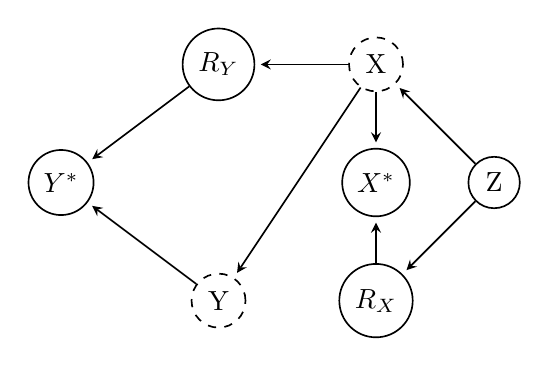
\begin{tikzpicture}[
            > = stealth, % arrow head style
            shorten > = 2pt, % don't touch arrow head to node
            auto,
            node distance = 3cm, % distance between nodes
            semithick % line style
        ]

\node[shape=circle,draw=black] (R_Y) at (0,0) {$R_Y$};
\node[shape=circle,draw=black, style=dashed] (Y) at (0,-3) {Y};
\node[shape=circle,draw=black] (Y^*) at (-2,-1.5) {$Y^*$};
\node[shape=circle,draw=black, style=dashed] (X) at (2,0) {X};
\node[shape=circle,draw=black] (X^*) at (2,-1.5) {$X^*$};
\node[shape=circle,draw=black] (R_X) at (2,-3) {$R_X$};
\node[shape=circle,draw=black] (Z) at (3.5,-1.5) {Z};

 \path [->] (X) edge node[left] {} (R_Y);
 \path [->] (X) edge node[left] {} (Y);
 \path [->] (Y) edge node[left] {} (Y^*);
 \path [->] (R_Y) edge node[left] {} (Y^*);
 \path [->] (X) edge node[left] {} (X^*);
 \path [->] (R_X) edge node[left] {} (X^*);
  \path [->] (Z) edge node[left] {} (X);
   \path [->] (Z) edge node[left] {} (R_X);
\end{tikzpicture}
\caption{A three variable MNAR m-graph} \label{fig:MNAREX}
\end{figure}

Consider the m-graph in figure 3.2. We notice that the one fully observed variable $Z$ does not d-separate $(R_X, R_Y)$ from $(X,Y)$ and therefore conclude that this m-graph corresponds to an MNAR missingness structure. However, we do have some relevant d-separations:

\begin{enumerate}
\item $X \dsep R_X | Z$
\item $Y \dsep (R_Y, R_X, Z) | X$
\end{enumerate}

Now, by the law of total probability and the chain rule for probability, we get that:

\begin{align*}
P(x,y) &= \sum_z P(x,y, z) \\
&= \sum_z P(x,y | z) P(z) \\
&= \sum_z P(y | x,z) P(x | z) P(z)
\end{align*}

When we apply our d-separations, we get that $P(y | x, z, R_Y = 0, R_X = 0) = P(y^*| x^*)$ and $P(x^*|z, R_X = 0) = P(x | z)$ and therefore:

$$\sum_z P(y | x,z) P(x | z) P(z) = \sum_z P(y^* | x^*,z, R_Y = 0, R_X = 0) P(x^* | z, R_X = 0) P(z)$$

So, we have succeed: the marginal distribution $P(x,y)$ is expressible as a sum and product of distributions which are recoverable simply using the d-separations, and so $P(x,y)$ is recoverable by theorem 4.
\end{example}

The second theorem aims a little higher: necessary \emph{and} sufficient conditions for recovering the full joint distribution $P(v_o, v_m)$.

\begin{theorem}
Given a m-graph G with no edges between $R$ nodes the joint distribution $P(v_o, v_m)$ can be recovered if and only if there is no variable $X \in V_m$ such that:
\begin{enumerate}
\item $X$ and $R_X$ are neighbors

\item $X$ and $R_X$ are connected by a path in which all intermediate nodes are colliders and elements of $V_m \cup V_o$ (i.e. at least partially observed, not an $R$ node, and not a proxy).
\end{enumerate}

When neither of these conditions apply, the joint $P(v_m, v_o)$ is recovered as:

$$\frac{P(v, R=0)}{\prod_i P(R_i = 0 | Mb(R_i), R_{Mb(R_i)} = 0)}$$

Where $Mb(R_i)$ is any \textbf{Markov blanket} for $R_i$: a set of nodes $Mb(R_i)$ such that \newline $R_i \dsep \mathbf{V} \backslash \{R_i, Mb(R_i)\} | Mb(R_i)$. In many cases, this will simply be $PA_{R_i}$. Similarly, $R_{Mb(R_i)}$ is the set of $R$ variables associated with the elements of $Mb(R_i)$ \citep{Mohan_2019}.
\end{theorem}

This final expression is a little difficult to parse, so we clarify what each component means in the following example.
\begin{example}
Lets return to the m-graph described in the previous example (figure 3.4). We check the two conditions laid out in the theorem:

\begin{enumerate}
\item The two variables subject to missingness, $Y$ and $X$ both lack an edge to their corresponding missingness node, and so the first condition is satisfied.

\item The only colliders in the graph are the two proxy nodes: $X^*$ and $Y^*$. Therefore, no path contains a collider which is an element of $V_o \cup V_m$.
\end{enumerate}

So, the population level joint $P(x,y,z)$ may be recovered as given in the theorem. This gives:

$$P(x,y,z) = \frac{P(x,y,z, R_X = 0, R_Y = 0)}{P(r_X | z)P(r_Y | x, R_x = 0)}$$
\end{example}

\chapter{Earlier Approaches to Selection Bias and the Missing Data Problem}

In statistics and many related fields, forms of the effect we are calling "selection bias" and "missing data" have gone by many names. As we have seen,  the tendency for types of survey recipients to respond more or less than others - (non) response bias - falls neatly into the framework of selection bias. In epidemiology and biostatistics, Berkson's bias (sometimes Berkson's paradox) describes a phenomenon in which two conditions that are independent at the population level become dependent within a sample as a result of both conditions affecting the likelihood of sample inclusion. This too is a kind of selection bias, as is Neyman's bias which results from survivors of a disease being selected for study but not those who died from the disease. In fact there are far more names for particular selection biases than we can describe here \citep{Delgado_2008}. One explanation for this extensive and overlapping nomenclature is that prior to the widespread use of graphical models, it was difficult to give any concise definition of selection bias that was specific enough to be useful. Selection bias is essentially about a sample with a different distribution than the population, but when that non-representivity can come from so many places this characterization is hardly useful.

In this section we will review a handful of notable earlier approaches to defining, correcting, and recognizing selection bias that have appeared within the literature. The purpose here is two-fold. For one, the historical background is generally useful to anyone looking for a thorough treatment of the subject. More pointedly, we will use the examples of previous methods to argue for the utility of the causal/graphical formulation used in this paper, as well as interpreting the techniques in that light.


\section{Case Analysis}

The easiest and most obvious way of "addressing" missing data is to ignore units which have missing values. There are a couple of techniques that take this approach. These techniques are widely used in practice despite significant undesirable theoretical properties \citep{Little_1986} which we discuss. In some cases, the adverse effects might be small - such as when missingness is very uncommon - but in other cases such techniques dramatically bias the results. 

\subsection{Complete-case Analysis}
In "complete-case" analysis only rows which are complete - not missing \emph{any} values - are included in the analysis. This can be thought of as deleting any row which has a missing value. There are two main problems with this approach. The first has to do with the structure of the missingness. In any case other than MCAR, the most restrictive of our taxonomy, complete case analysis produces distributions different from the population distribution \citep{Little_1986}. This is because complete case analysis is essentially a process by which data subject to missingness is made into data affected by selection bias. Since we remove any rows with missing values, we can think about complete case analysis as the process of constructing a complete data set subject to selection. Particularly, in the new data set, $S= \begin{cases}1 \text{ if } R=0 \\ 0 \text{ if } R = 1 \end{cases}$ and so in the corresponding graph, and edge would exist between each parent of an $R$ node and the selection node. Therefore, only under MCAR do we have a graph with no edges between the selection node and the rest of the graph.

The second problem with complete-case analysis is that in many contexts, it is highly inefficient \citep{Little_1986}. Consider a survey with a large number of questions and suppose we wish to know the distribution of the respondents' answers to a particular question. To conduct a complete-case analysis in such a situation would mean throwing out every row in which the respondent had failed to answer any of the many questions, even if they had answered the question of interest. In such situations, complete-case analysis results in sample sizes which are far smaller than the sample size of the original data set. This, of course, has consequences for the power of statistical tests, the size of confidence intervals, etc. 

Despite these drawbacks, complete-case analysis is very common. As above, this is mathematically appropriate when data are MCAR, but this is often not the case. Nonetheless, complete case analysis may be "good enough" for some purposes, especially when the number of excluded rows is small enough that any reasonable values for the missing data in the column of interest are unlikely to dramatically affect the analysis \citep{Schafer_2002}.

\subsection{Available-case Analysis}

The inefficiency of complete-case analysis has an obvious (partial) remedy. Instead of deleting every row which is subject to missingness in any column, we first select the variables of interest and then only delete rows which are missing values in the corresponding columns. This method is called "available-case" analysis or sometimes "pairwise deletion". Of course, when the number of variables of interest is close to the overall number of variables this doesn't help much, but when only a couple are needed much more data can be preserved. However, this method does nothing to address the main theoretical problem of bias: once again, data which is not MCAR is generally not appropriate for available case analysis.

T

\section{Imputation based Techniques} 

Imputation is the process of "guessing" missing values such that an analysis can be performed on the imputed data set. Imputation methods vary widely in their simplicity and practicality \citep{Schafer_2002}. Broadly, imputation techniques fall into one of two categories: "single" imputation and "multiple" imputation. As the names suggest, the difference between the methods is that single imputation replaces missing values with a single imputed value whereas multiple imputation replaces missing values with multiple plausible values, effectively creating multiple datasets on which the analysis can be performed. We give an overview of both approaches.

\subsection{Single Imputation}
In single imputation, the task is to replace missing values with "reasonable" guesses. There are several techniques used to generate such values all of which rely on the missingness being MCAR or MAR. We summarize them below from simplest to most complex and then discuss their advantages and disadvantages. 

\begin{itemize}
\item Mean Imputation: For a variable $Y$ subject to missingness, the missing values are replaced with the mean of the observed values of $Y$ \citep{Little_1986}.

\item Hot Deck Imputation: For a variable $Y$ subject to missingness, the missing values are replaced with the value from another row. Sometimes, this row is chosen randomly, whereas other times the row is selected based on similarity of observed covariates \citep{Little_1986}, \citep{Schafer_2002}.

\item Regression Imputation: For a variable $Y$ subject to missingness, a model $f$ is formulated based on the fully observed variables $\mathbf{X}$ is formulated and trained on the rows in which $Y$ is observed. Then, the model prediction $\hat y_i = f(\mathbf{x}_i)$ is used to imputed each missing value of $Y$ \citep{Schafer_2002}.

\item Random Regression Imputation: Same as regression imputation except rather than replacing missing $y_i$ with $\hat y_i$ we replace it with $\hat y_i + \epsilon$ where $\epsilon$ is drawn from the regression noise distribution (e.g. a normal distribution centered at $0$ in the case of linear regression). Alternatively, the replacement value can be sampled from the posterior distribution of a Bayesian model \citep{Rubin_1996}.
\end{itemize}

In general, the methods at the end of this list are preferable to the methods at the beginning. Starting with mean imputation, there are two main problems. The first is that unless the data is MCAR, the conditional (on fully observed $\mathbf{X}$) expected value  of the replacement $E[y| \mathbf{x}]$ will in general be different from the unconditional mean $E[y]$ which is used to impute. This means that when the data is not MCAR, the estimates based on the imputed data will be biased. The other problem is that because the imputed values are all the same (the mean) the variance of the imputed column will be deflated \citep{Gelman_2006}. This occurs regardless of three structure of the missingness.

Hot-deck imputation attempts to solve this problem by adding noise in the form of 

\subsection{Multiple Imputation}

The problems with single imputation methods led researchers to search for more sophisticated techniques. Donald Rubin introduced first introduced the concept in 1977 \citep{Rubin_1977}but its classic treatment is Rubin's 1987 book on the topic. 

\section{The Heckman Correction}
James Heckman's well-cited 1979 paper "Sample Selection Bias as a Specification Error" proposes a method for overcoming selection bias that is among the most prominent selection adjustment techniques \citep{Heckman_1979}. Heckman was an economist, and his correction technique comes in the context of economic modeling, particularly linear regression models. Because it is situated within this framework, the correction is parametric - it requires the  assumption of normally distributed noise. We consider the situation in the response variable is missing for some observations. Since we are interested modeling the population values and coefficients, this poses a potential problem. The title of Heckman's paper gives a hint to his strategy: specification error refers to the omission of a relevant variable from a model. 

The method proceeds in two parts: first, a model is constructed for sample inclusion and second, an expected error term is calculated such that it can be included in the regression model to remove the bias associated with its exclusion. We now describe Heckman's method in detail.

\subsection{Premise}

Heckman's original paper is concerned with estimating model coefficients in the context of a finite sample. So far, we have been considering distributions rather than samples, and for the sake of continuity (as well as avoiding excess indexing) we will present the method in the context of distributions. Fortunately, the math is essentially the same.

Assume that we have access to the distributions of a dependent variable $Y$, a vector of regressor variables $\mathbf{X}$, and a normally distributed noise term $\epsilon$ which is independent of $\mathbf{X}$. Further assume that the linear regression assumption holds, i.e.

$$Y = \mathbf{X} \boldsymbol{\beta} + \epsilon.$$

Now, assuming we have the joint distribution $P(y, \mathbf{x}, \epsilon)$ we can get $\mathbf{\beta}$ using standard techniques. However, if a selection mechanism is present, this may not be possible. Unlike the selection mechanisms we saw in the previous chapter, the mechanism only causes values for $Y$ to be missing - i.e. $(X, s)$ is measured in the population but $Y$ is only measured when $S = 1$. Heckman's correction can be applied when the selection mechanism follows a specific form. Particularly, assume that there is another set of random variables that also follow the linear model pattern: 

$$Z = \mathbf{W} \boldsymbol{\delta} + \tau.$$

Again, $\mathbf{W}$ is a vector of regressors, $\boldsymbol{\delta}$ is a coefficient vector and $\tau$ is normally distributed and independent of $\mathbf{W}$. Oftentimes, it is the case  that $\mathbf{W}$ contains the regressors in $\mathbf{X}$, but this is not needed. In general, $Z$ is not measured at all, but as with $\mathbf{X}$, $(\mathbf{W}, s)$ is measured in the population. We also require that the joint $P(\tau, \epsilon)$ follows the bivariate normal distribution. Heckman's correction can be applied when the selection mechanism is of the form:

$$S = I(Z > c) = I( \mathbf{W} \boldsymbol{\delta} + \tau > c).$$ 

For some constant $c$. Without losing generality, we assume that $c = 0$. So selection occurs when a second random variable, $Z$,  passes a particular threshold. 

\subsection{Implementing the Correction}

Heckman is viewing selection bias as being the result of an omitted variable which we can obtain. Here we give the derivation of what this variable actually is, closely following the original paper but with some clarifications and changes to notation as in \citep{Jin}. We know that:

$$E[Y | \mathbf{X}, S = 1] = E[ \mathbf{X} \boldsymbol{\beta} + \epsilon | \mathbf{X}, S = 1] = \mathbf{X} \boldsymbol{\beta} + E[\epsilon |  \mathbf{X}, S = 1].$$

Our independence assumption gives that $ E[\epsilon |  \mathbf{X}, S = 1] =  E[\epsilon |  S = 1]$ and so this is the quantity we wish to estimate. Now, $S=1 \implies  \mathbf{W} \boldsymbol{\delta} + \tau > 0$ and we write:  

$$E[\epsilon |  \mathbf{X}, S = 1] = E[\epsilon | \mathbf{W} \boldsymbol{\delta}+ \tau > 0] = E[\epsilon |  \tau > - \mathbf{W} \boldsymbol{\delta}].$$

Since $(\epsilon, \tau)$ follows a bivariate normal distribution and each have a marginal mean of $0$, the conditional expectation $E[\epsilon | \tau] = \rho \frac{\sigma_{\epsilon}}{\sigma_{\tau}} \tau$ where $\rho$ is the correlation between $\epsilon$ and $\tau$ and $\sigma^2_{\epsilon}$, $\sigma^2_{\tau}$ are the respective variances. Let $\gamma  = \rho \frac{\sigma_{\epsilon}}{\sigma_{\tau}}$ giving $E[\epsilon | \tau] = \gamma \tau$. Notice that when $\rho = 0$ (meaning $\epsilon$ and $\tau$ are independent), the $\gamma$ term is equal to $0$ and therefore the selection does not bias the estimate.  We may then apply the law of total expectation (sometimes call Adam's law):

$$E[\epsilon | \tau] = E[E[\epsilon | \tau] | \tau] = E[\gamma \tau | \tau] = \gamma E[\tau | \tau]$$	

So, when $\tau > - \mathbf{W} \boldsymbol{\delta}$, $E[\tau | \tau] = E[\tau | \tau > - \mathbf{W} \boldsymbol{\delta}]$ and we have that:

$$E[\epsilon | \tau >  - \mathbf{W} \boldsymbol{\delta}]  = \gamma E[ \tau | \tau >   - \mathbf{W} \boldsymbol{\delta}]$$																																																												
We recognize this as the expectation of a truncated normal, which is given by the inverse Mills ratio $E[X | X > x] = \sigma \frac{\phi(\frac{x- \mu}{\sigma})}{1 - \Phi(\frac{x - \mu}{\sigma})}$ for $X \sim N(\mu, \sigma^2)$. As usual, $\phi$ is the density function for the standard normal and $\Phi$ is the distribution function. By assumption, $\mu = 0$. Therefore,						

$$E[\epsilon | \tau > -\mathbf{W} \boldsymbol{\delta}] = \gamma \sigma_{\tau}\frac{\phi(\frac{-\mathbf{W} \boldsymbol{\delta}}{\sigma_\tau})}{1 - \Phi(\frac{-\mathbf{W} \boldsymbol{\delta}}{\sigma_\tau})}.$$				

So the bias term  we want to estimate is $\gamma\sigma_{\tau}\frac{\phi(\frac{-\mathbf{W} \boldsymbol{\delta}}{\sigma_\tau})}{1 - \Phi(\frac{-\mathbf{W} \boldsymbol{\delta}}{\sigma_\tau})}$. This is done in several parts \cite{Heckman_1979}.

\begin{enumerate}
\item  First, a probit model is employed to estimate $\frac{\boldsymbol{\delta}}{\sigma_\tau}$, i.e. $P(S = 1 | \mathbf{W}) = \Phi(\frac{ \mathbf{W} \boldsymbol{\delta}}{\sigma_{\tau}})$. 

\item This estimated quantity is used to get an estimate of  $\frac{\phi(\frac{-\mathbf{W} \boldsymbol{\delta}}{\sigma_\tau})}{1 - \Phi(\frac{-\mathbf{W} \boldsymbol{\delta}}{\sigma_\tau})}$.

\item The estimate of $\frac{\phi(\frac{-\mathbf{W} \boldsymbol{\delta}}{\sigma_\tau})}{1 - \Phi(\frac{-\mathbf{W} \boldsymbol{\delta}}{\sigma_\tau})}$ is included in the corrected model $Y = \mathbf{X} \boldsymbol{\beta} + \frac{\phi(\frac{-\mathbf{W} \boldsymbol{\delta}}{\sigma_\tau})}{1 - \Phi(\frac{-\mathbf{W} \boldsymbol{\delta}}{\sigma_\tau})} + \epsilon$. The coefficient on $\frac{\phi(\frac{-\mathbf{W} \boldsymbol{\delta}}{\sigma_\tau})}{1 - \Phi(\frac{-\mathbf{W} \boldsymbol{\delta}}{\sigma_\tau})}$ is then an estimate of $\gamma \sigma_\tau = \rho \sqrt{\sigma_\epsilon}$. In this model, the estimate of the intercept,$\hat \beta_0$, is now consistent, meaning that as the sample size increases $\hat \beta_0 \rightarrow \beta_0$ in probability.
\end{enumerate}

Something to note: unlike the approach we see in the more contemporary selection bias literature, Heckman's method asks for external information on the selection mechanism itself, not the variables being measured. In addition to this, Heckman makes very strong parametric assumptions. Sometimes when such assumptions are made, the method is still relatively robust to (mild) violations.  However, Heckman's correction's does not generally have this property, and violations of the set-up can cause seriously biased estimates \citep{Little_1986}. This lack of robustness has led to Heckman's method becoming less popular in recent years \citep{Bushway_2007}.


\subsection{Graphing Heckman}
Although Heckman's method makes assumptions which are not captured by a causal graph (such as normality of $\epsilon$, $\tau$), it is still instructive to supply the graph that Heckman's setup induces. 

\begin{figure}[H]
\begin{center}
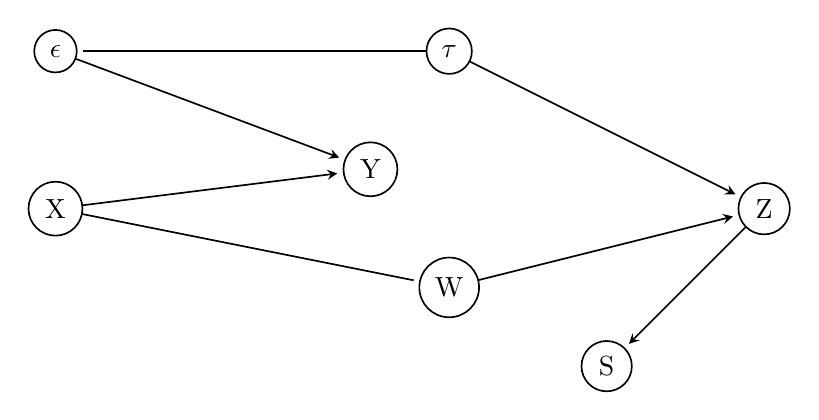
\begin{tikzpicture}[
            > = stealth, % arrow head style
            shorten > = 2pt, % don't touch arrow head to node
            auto,
            node distance = 3cm, % distance between nodes
            semithick % line style
        ]
\node[shape=circle,draw=black] (X) at (0,0) {X};
\node[shape=circle,draw=black] (Y) at (4,.5) {Y};
\node[shape=circle,draw=black] (Z) at (9,0) {Z};
\node[shape=circle,draw=black] (S) at (7,-2) {S};
\node[shape=circle,draw=black] (W) at (5,-1) {W};
\node[shape=circle,draw=black] (E) at (0,2) {$\epsilon$};
\node[shape=circle,draw=black] (T) at (5,2) {$\tau$};

 \path [->] (X) edge node[left] {} (Y);
 \path [->] (E) edge node[left] {} (Y);
  \path [->] (T) edge node[left] {} (Z);
    \path [->] (W) edge node[left] {} (Z);
        \path [->] (Z) edge node[left] {} (S);
   \path [-] (T) edge node[left] {} (E);
   \path [-] (X) edge node[left] {} (W);
\end{tikzpicture}
\end{center}
\caption{PDAG corresponding to the structural equations in Heckman's set up. We leave arrows off the edges between $\epsilon$ and $\tau$ and between $X$ and $W$ since the directions are not given by the structural equations.}
\end{figure}

One fact we observed earlier that this image makes clear is that when the edge between $\epsilon$ and $\tau$ is inactive, the sampling procedure will not affect the estimates since $Y \dsep_G S | X$ and so $P(y| x) = P(y|x, S = 1)$. Visualization the structure this way also leads to the conclusion that if the joint distribution $(\mathbf{X},Z)$ is measured in the population, we can use Barenboim's second theorem to recover $P(y|x)$. Of course, this is not the usual case since $Z$ is typically not measured at all, much less in the population.



\subsection{Examples}

Heckman developed his technique in the context of economic research, and its implementation typically relies on further assumptions justified by economic theory. Particularly, $Z$ is often understood as an \emph{unmeasured} continuous random variable following the linear regression assumptions \citep{Winship_Mare_1992}. Sometimes,  this variable is not directly measurable - such as an individual propensity or ability - that is nonetheless assumed to exist. We quickly review a number of  fairly standard  examples used to introduce Heckman's method \citep{Heckman_1979}, \citep{Guo_2015}.

\begin{enumerate}
\item Estimating the wages women not in the workforce would make if they entered the workforce using data for women currently in the workforce. Selection occurs because the women in the workforce differ from those who are not.

\item Estimating the effect of unionization of worker wages - similar to the last example, unionized workers might have joined the union because they were unsatisfied with their wages pre-unionization.

\item Estimating effects of schooling/training programs of worker productivity. Once again, the problem is that the people who choose to participate in such programs cannot be used to represent the workers who did not make that 
\end{enumerate}

In the spirit of some of these examples, we describe a relevant variation in more detail. Suppose that we are working with Reed College academic services to measure the effect of tutoring on student homework grades in the introductory chemistry sequence. We have collected a collected a set of relevant covariates ($\mathbf{X}$) on all students in the course such as major, high school grades, basic demographics, etc. The response variable ($\text{Grade Change}$) is the difference between the student's average homework scores before their first tutoring appointment and the average score after. Since some students do not seek tutoring, their value of $Y$ is missing. We assume that the response variable follows the linear regression assumptions:

$$\text{Grade Change} =   \mathbf{X}\boldsymbol{\beta} + \epsilon$$

For normally distributed $\epsilon$ with mean $0$. As students who participate in tutoring might differ from students who do not, it would be incorrect to use the model created using data for students that did seek tutoring to estimate the impact that tutoring would have on students who did not chose to be tutored. So, we must create a model for a student's probability of going to tutoring. To do this though Heckman's technique, we must further assume that a student seeks tutoring a when some unmeasured value crosses a threshold. There are multiple options here, and in practice this a stage that requires existing economic theory to be justified. In our case, these details are not important we assume that $\text{Tutoring Value}$ is, for each student, the perceived value of going to tutoring minus the students value of an equal amount of time for a different activity, such that a student goes to tutoring if  $\text{Tutoring Value}$ is positive. We have further collected from each student covariates capturing their motivation to do well in their courses, their perception of the usefulness of tutoring, and the amount of free time they have. Together with the covariates we measured for $X$, these variables constitute $\mathbf{\mathbf{W}}$,  and again we require linear regression assumptions are satisfied:

$$\text{Tutoring Desire} = \mathbf{W}  \boldsymbol{\delta} + \tau$$

With $\tau$ being normally distributed with mean $0$ such that $\epsilon$ and $\tau$ are jointly bivariate normal with correlation $\rho$. We can then implement the correction as follows:

\begin{enumerate}
\item Define the selection variable $S$ as $1$ for student with data for $\text{Grade Change}$ and $0$ for those who do not.

\item Create a probit model $P(S=1 | W)$ which yields as estimate of $\frac{\boldsymbol{\delta}}{\sigma_\tau}$ as the coefficients on $\mathbf{W}$.

\item We then estimate the inverse Mill's ratio $\frac{\phi(\frac{-\mathbf{W} \boldsymbol{\delta}}{\sigma_\tau})}{1 - \Phi(\frac{-\mathbf{W} \boldsymbol{\delta}}{\sigma_\tau})}$ and include the term in the regression equation, giving consistent estimates of $E[\text{Grade Change} | \mathbf{X}]$.
\end{enumerate}



\section{Probability and Propensity Weighting}

Another technique worth mentioning is a very general approach called inverse probability weighting (IPW) which has applications for both selection bias and missing data. Versions of the technique are old  and have uses well outside of adjusting for selection bias or missing data \citep{Horvitz_1952}, but we give an interpretation particularly suited for these tasks. Given a particular (non-representative or partially observed) sample, the goal is to construct a 'new' sample which follows the population distribution by weighting each element of the existing sample by its probability of having been sampled/missing. Doing this requires knowing something about the selection rule, particularly knowing the probability that any particular set of values is sampled \cite{Cortes_2008}. Like Heckman's method, IPW is for correcting the bias of an estimator rather than a distribution. However, as we will see, a related technique can be used to recover biased distributions. 

Probability weighting techniques are associated with adjusting for confounding bias for causal inference, but methods have been developed that address selection bias as well \citep{Correa_2017}.

To build intuition, consider the simple case of trying to estimate mean of a finite set of values  $x_1,x_2,...,x_n$ using a sample. We take a sample (i.i.d. with replacement) $X_1,...,X_n$ but the values are not sampled with equal probabilities, rather, $P(X_1 = x_i) = p_i > 0$ for all $j$ (with $\sum p_i = 1$). By the definition of expectation, $E[X_i] = \sum_{i=1}^n p_i x_i$ which in general is not equal to $\frac{1}{n}\sum_{i=1}^n x_i$. For our purposes, the uniform distribution $P(X_1 = x_i) = \frac{1}{n}$ for all $i$ is the \emph{target distribution} - or the distribution that we would like to be sampling from. However, if we know the values of $p_i$, we can re-weight each $x_i$ by multiplying by the product of the probabilities under the target distribution and the probabilities under the sampling distribution giving $x_i' = \frac{x_i}{np_i}$. Then, when we sample from $x_1', x_2', ..., x_n'$ according to $p_1,...,p_n$ as $X_1', X_2', ..., X_n'$ we get $E[X_i'] = \sum_{i=1}^n x_i' p_i = \sum_{i=1}^n  \frac{x_i}{n p_i} p_i = \frac{1}{n} \sum_{i=1}^n x_i$. 

This method of estimating the mean from a biased sample is one of the earliest methods of adjusting for selection bias and is called the Horvitz-Thompsom estimator \citep{Little_1986}. Of course, inverse probability weighting can be applied in a more general context than estimating the mean of a population. When an estimator is


\subsection{Propensity Scores}

As with Heckman's two-step estimator, inverse probability weighting is can be used to address the "missing data" problem in which covariates are measured for some observations but the response is missing for some units. Inverse probability weighting is also sometimes used when treatments are assigned non-randomly \citep{Haneuse_2009}.  In both of these cases, a model (such as probit or logit) can be constructed to estimate probability of missingness or treatment for any particular entry, and thereby the weights may be estimated. The estimated probability of being sampled, $\hat\{P(S = 1 | \mathbf{x})\}$ is referred to as a \emph{propensity score}. In this case, the method is typically called propensity score weighting \citep{Bishop_2018}. 


\subsection{Inverse Probability Weighting for Distributions}

For most of this paper, our primary concern is recovering entire distributions affected by selection bias rather than making a particular estimator consistent. In this case, a similar technique which also relies on $P(S=1 | \mathbf{v})$ can be applied. 

When dealing with distributions affected by selection bias, our target distribution is $P(\mathbf{v})$ and we have access to $P(\mathbf{v} | S = 1)$. Then, Bayes rule gives that \citep{Cortes_2008}:

$$P(\mathbf{v}) = \frac{P(\mathbf{v}  | S = 1)P(S = 1)}{P(S=1 | \mathbf{v})} = P(\mathbf{v}  | S = 1) \frac{P(S = 1)}{P(S=1 | PA_{S})}$$

So, with knowledge of $P(S=1 | PA_S)$ and $P(S = 1)$ we can fully recover $P(\mathbf{v})$ by again multiplying by the target distribution. 


So clearly knowing $P(S = 1)$ and $P(S = 1|x)$ is quite powerful. As with Heckman, this method requires information about the selection mechanism, but doesn't assume population level information about the other variables. This is a real difference between inverse probability weighting or the Heckman correction and the graphical approaches we examine next. However, unlike Heckman, inverse probability weighting does not require  assumptions about the parametric structure of the data and instead works with non-parametric values.   We give a brief example drawing on our previous discussion of the 1936 Literary Digest survey.

\subsection{}

Consider the first explanation of the Literary Digest's survey failure: that selection based on SES (via ownership of a telephone/car) was solely responsible for the non-representivity of the sample. We are interested in the mean of $C$, that is, the probability that a randomly selected voter will cast their ballot for Roosevelt. 


\begin{figure}
\begin{center}
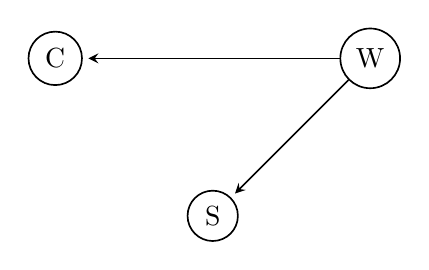
\begin{tikzpicture}[
            > = stealth, % arrow head style
            shorten > = 2pt, % don't touch arrow head to node
            auto,
            node distance = 3cm, % distance between nodes
            semithick % line style
        ]
\node[shape=circle,draw=black] (C) at (0,0) {C};
\node[shape=circle,draw=black] (W) at (4,0) {W};
\node[shape=circle,draw=black] (S) at (2,-2) {S};

 \path [->] (W) edge node[left] {} (S);
 \path [->] (W) edge node[left] {} (C);

\end{tikzpicture}
\end{center}
\caption{Graph corresponding to selection bias based on income} 
\end{figure}

\section{Getting Graphical}


By the first decade of the 2000's, Pearl's causality framework had become well-known not just in computer science but in applied fields as well. Accordingly, this period marks the first attempts to formulate selection bias in graphical terms. Specifically, we discuss two influential papers that drawn on Pearl's work.

\subsection{Hern\'an et. al}

Miguel Hern\'an's 2004 paper "A Structural Approach to Selection Bias" sets out to distinguish between selection bias and other problematic features of studies using the logic of causality. Although some other work had used DAGs to represent selection into a study \citep{Robbins_2001}, \citep{Pearl_1995}, Hern\'an's paper went further in that it gave an explicitly graphical interpretation of presence bias caused by selection. Hern\'an, an epidemiologist, is particularly concerned with presence of selection bias within case-control and cohort studies, and his paper proceeds primarily by drawing on examples of such studies in which selection bias is a problem. As is often the case in medical studies, the random variables considered are mostly binary, meaning that instead of looking for conditional distributions in general, related quantities such as risk ratios or odds ratios are considered. However, the concepts are very similar.

The core of Hern\'an's argument is that selection bias occurs when we \emph{condition on common effects} of the exposure (treatment) and the outcome through selection. That is, the effect of the treatment $X$ on the outcome $Y$ is affected by selection bias when both selection and the treatment depend on $X$ or an ancestor (cause) of $X$.  In Barenboim's  2014 paper, we saw a version of this statement in theorem 1: $P(y|\mathbf{x})$ is recoverable as $P(y|\mathbf{x}, S = 1)$ when $Y \dsep_G S | X$. By the definition of d-separation,  This definition can be contrasted with confounding, which has its roots in common \emph{causes}. Hern\'an gives an simple example illustrating what is meant by this which we reproduce. 

\begin{figure}[H]
\begin{center}
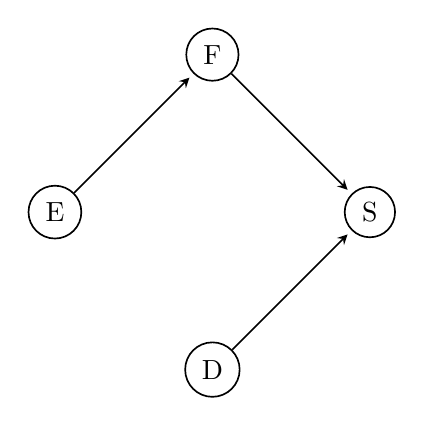
\begin{tikzpicture}[
            > = stealth, % arrow head style
            shorten > = 2pt, % don't touch arrow head to node
            auto,
            node distance = 3cm, % distance between nodes
            semithick % line style
        ]
\node[shape=circle,draw=black] (E) at (0,0) {E};
\node[shape=circle,draw=black] (F) at (2,2) {F};
\node[shape=circle,draw=black] (D) at (2,-2) {D};
\node[shape=circle,draw=black] (S) at (4,0) {S};


 \path [->] (E) edge node[left] {} (F);
 \path [->] (D) edge node[left] {} (S);
  \path [->] (F) edge node[left] {} (S);
\end{tikzpicture}
\end{center}
\caption{Study design for the Hern\'n's example}
\end{figure}

Here, $E$ is the treatment, estrogen supplements, $F$ denotes women who fractured their hips, and $D$ represents having a heart attack. We want to know if estrogen use increases the risk of having a heart attack. The study participants were gathered in such that the controls, the women who did not have a heart attack, were disproportionately women who had fractured their hips. This could be because the sample was taken from a particular hospital. Since estrogen use decreases a woman's risk of breaking her hip, this means that women taking estrogen are underrepresented within the controls. So, if we look at $P(d | e, S = 1)$ then we will find a positive relationship between $F$ and $E$ since selection into the study is a caused by both estrogen use (indirectly through decreased hip factors) and having a heart attack. So by selecting our sample in the way that we have, we have conditioned on a common effect of both the treatment and the outcome, biasing our inferences. In the reader's digest survey, 

Although Hern\'an's work was important in categorizing selection bias through graph structure, the paper was not primarily concerned with correcting for selection bias. There is a short section on how to overcome such bias, but it was limited to inverse probability weighting, a technique we have already discussed. Fortunately, the next paper we examine does. 



\subsection{Geneletti et. al}

Following up on Hern\'an's work characterizing selection bias, another epidemiologist, Sara Geneletti and her co-authors give a method for correcting selection bias in retrospective case-control studies using DAGs and conditional independence \citep{Geneletti_2008}. In spirit this is very similar to Bareinboim's work but limited to a specific study design such that further assumptions can be leveraged.  We now briefly review the structure of a retrospective case-control study. 

Unlike experiments where treatments are assigned randomly and outcomes measured after treatment, or cohort studies where individuals are tracked over a long period to see if they develop a disease, retrospective case-control studies (often just called case-control studies) select individuals for sample inclusion \emph{after} they have contracted a disease \citep{Woodward_1999}. Two groups are selected: one which has a particular disease/condition and one which does not. Then, covariates are gathered for both groups, with the hope of discovering some factors which are more common in one group that the other. So for instance, we could gather a sample of lung cancer patients and another of adults without lung cancer. We would likely discover that after adjusting for relevant demographic factors (age, sex, SES, etc.) smoking was more common in the lung cancer group and then construct an estimate of the risk ratio for smoking and lung cancer. However, this kind of study is particularly susceptible to selection bias \citep{Woodward_1999} \citep{Geneletti_2008}. This can happen for different reasons, but one of most prominent is that the treatment (smoking, in our example) might cause patients to be admitted to the hospital for a reason unrelated to lung cancer, but upon their admission be discovered to have lung cancer. In this way, we might see a dependence between lung cancer and smoking that is caused by smoker's greater likelihood to be diagnosed.  Similarly, when both cases and controls are selected from the hospital Berkson's bias could create a false negative association \citep{Hernan_2004}.  

Much like the first theorem of \cite{Bareinboim_2014}, Geneletti goes about recovering a conditional distribution by constructing a "bias breaking" set that d-separates (though she does not use the term) the selection node from treatment. The paper uses nearly the same example as Hern\'an's but here an edge exists between $E$ and $D$, meaning e


\begin{figure}[H]
\begin{center}
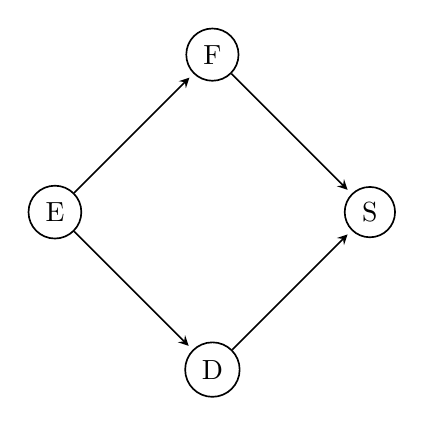
\begin{tikzpicture}[
            > = stealth, % arrow head style
            shorten > = 2pt, % don't touch arrow head to node
            auto,
            node distance = 3cm, % distance between nodes
            semithick % line style
        ]
\node[shape=circle,draw=black] (E) at (0,0) {E};
\node[shape=circle,draw=black] (F) at (2,2) {F};
\node[shape=circle,draw=black] (D) at (2,-2) {D};
\node[shape=circle,draw=black] (S) at (4,0) {S};


 \path [->] (E) edge node[left] {} (F);
 \path [->] (D) edge node[left] {} (S);
   \path [->] (E) edge node[left] {} (D);
  \path [->] (F) edge node[left] {} (S);
\end{tikzpicture}
\end{center}
\caption{Study design for the Geneletti's example}
\end{figure}



\section{Set-up}

In Chapter 2 we discussed the contributions of a group of current researchers on the topic of selection bias. Barenboim, Correa, Tian, and Pearl have made decisive progress in characterizing selection bias graphically and giving conditions for recoverability with or without unbiased (population level) data. However, there are cases in which 
%If you feel it necessary to include an appendix, it goes here.


%This is where endnotes are supposed to go, if you have them.
%I have no idea how endnotes work with LaTeX.

  \backmatter % backmatter makes the index and bibliography appear properly in the t.o.c...

% if you're using bibtex, the next line forces every entry in the bibtex file to be included
% in your bibliography, regardless of whether or not you've cited it in the thesis.
    \nocite{*}

% Rename my bibliography to be called "Works Cited" and not "References" or ``Bibliography''
% \renewcommand{\bibname}{Works Cited}

%    \bibliographystyle{bsts/mla-good} % there are a variety of styles available; 
%  \bibliographystyle{plainnat}
% replace ``plainnat'' with the style of choice. You can refer to files in the bsts or APA 
% subfolder, e.g. 
 \bibliographystyle{APA/apa-good}  % or
 \bibliography{thesis}
\nocite{*}% there are a variety of styles available; 
%  \bibliographystyle{plainnat}
% replace ``plainnat'' with the style of choice. You can refer to files in the bsts or APA 
% subfolder, e.g. 
%\bibliographystyle{APA/apa-good}  % or
 % Comment the above two lines and uncomment the next line to use biblatex-chicago.
 %\printbibliography[heading=bibintoc]
\appendix
\chapter{Appendix}

\section{Heckman}
\subsection{Conditional Expectation of Bivariate Normal Distribution}

We want to show that for $(\epsilon, \tau) \sim N((0,0), \boldsymbol{\Sigma})$ (where $\boldsymbol{\Sigma} = \begin{pmatrix}
\sigma_\epsilon^2 &\ \rho \sigma_\epsilon \sigma_\tau \\
\rho \sigma_\epsilon \sigma_\tau &\ \sigma_\tau^2
\end{pmatrix}$ and $\rho$ is the correlation of $\epsilon$ and $\tau$) the conditional $E[\epsilon | \tau] = \rho \frac{\sigma_\epsilon}{\sigma_\tau} \tau$. The normal distribution has the property that the covariance (therefore correlation) of determines the dependence structure. Consider the random variable $\epsilon - \frac{\rho}{\sigma_\tau} \tau$. We want to show that this random variable is independent of $\tau$. This is true when their covariance is $0$, i.e. when $E[\tau (\epsilon -\rho \frac{\sigma_\epsilon}{\sigma_\tau}\tau)] - E[\tau] E[\epsilon - \rho \frac{\sigma_\epsilon}{\sigma_\tau}  \tau] = 0$. In fact, since $E[\tau]=0$ by assumption, we want to show that $E[\tau (\epsilon -\rho \frac{\sigma_\epsilon}{\sigma_\tau} \tau)] = 0$

We have:

\begin{align*}
E[\tau (\epsilon - \rho \frac{\sigma_\epsilon}{\sigma_\tau} \tau)] &= E[\tau \epsilon] -  \rho \frac{\sigma_\epsilon}{\sigma_\tau} E[\tau^2] \\
&=  \rho \sigma_\tau \sigma_\epsilon -  \rho \frac{\sigma_\epsilon}{\sigma_\tau}E[\tau^2] \\ 
&= \rho \sigma_\tau \sigma_\epsilon -  \rho \sigma_\tau \\
&= 0
\end{align*}
As desired. Then, applying independence, we have that:

\begin{align*}
E[\epsilon | \tau] &= E[\epsilon - \frac{\rho}{\sigma_\tau} \tau +  \frac{\rho}{\sigma_\tau} \tau | \tau] \\
&= E[\epsilon - \rho \frac{\sigma_\epsilon}{\sigma_\tau} \tau | \tau] + E[\rho \frac{\sigma_\epsilon}{\sigma_\tau} \tau | \tau] \\
&= E[\epsilon - \rho \frac{\sigma_\epsilon}{\sigma_\tau} \tau] +\rho \frac{\sigma_\epsilon}{\sigma_\tau}E[\tau | \tau] \\
&= E[\epsilon] + \rho \frac{\sigma_\epsilon}{\sigma_\tau} \tau \\
&= \rho \frac{\sigma_\epsilon}{\sigma_\tau} \tau. 
\end{align*}

\subsection{Truncated Normal and the Inverse Mills Ratio}

We show that $E[\tau | \tau \geq t] = \sigma_\tau \frac{\phi(t)}{1 - \Phi(t)}$. By the definition of truncated density, the truncated PDF $f_{\tau | \tau > t}$ is:

$$f_{\tau | \tau > t}(x) = \frac{f_\tau(x)}{1 - F_\tau(t)} \text{  for } x > t$$

Where $f$ is the density function for $\tau$ and $F$ is the distribution function for $\tau$. In particular, these are $f(x) = \frac{1}{\sigma_\tau} \phi(\frac{x}{\sigma_\tau})$ and $F(x) = \Phi(\frac{x}{\sigma_\tau})$ giving $f_{\tau | \tau > t}(x) = \frac{\phi(\frac{x}{\sigma_\tau})}{\sigma_\tau(1 - \Phi(\frac{t}{\sigma_\tau}))} \text{  for } x > t$. To find the expected value, we integrate. 

\begin{align*}
E[\tau | \tau > - t] &= \int_t^\infty x f_{\tau | \tau > t}(x) \\
&= \int_t^\infty \frac{\phi(\frac{x}{\sigma_\tau})}{\sigma_\tau(1 - \Phi(\frac{t}{\sigma_\tau}))} \\
&= \frac{1}{\sigma_\tau(1 - \Phi(\frac{t}{\sigma_\tau}))} \int_t^\infty x \phi(\frac{x}{\sigma_\tau})  \\
&= \frac{1}{\sigma_\tau(1 - \Phi(\frac{t}{\sigma_\tau}))} \int_t^\infty  \frac{x}{\sigma_\tau \sqrt{2 \pi}}e^{-\frac{x^2}{2 \sigma_\tau^2}} \\
&= \frac{1}{\sigma_\tau(1 - \Phi(\frac{t}{\sigma_\tau}))} \left( -\dfrac{{\sigma_\tau}e^{-\frac{x^2}{2{\sigma_\tau}^2}}}{\sqrt{{2\pi}}} \bigg |_t^\infty \right) \\
&= \frac{1}{\sigma_\tau(1 - \Phi(\frac{t}{\sigma_\tau}))} \dfrac{{\sigma_\tau}e^{-\frac{t^2}{2{\sigma_\tau}^2}}}{\sqrt{{2\pi}}}  \\
&= \frac{\sigma_\tau^2 \phi(\frac{t}{\sigma_\tau})}{\sigma_\tau(1 - \Phi(\frac{t}{\sigma_\tau}))} \\
&= \sigma_\tau  \frac{\phi(\frac{t}{\sigma_\tau})}{(1 - \Phi(\frac{t}{\sigma_\tau}))} 
\end{align*}
Which is the desired result.


% Finally, an index would go here... but it is also optional.
\end{document}
